% ----------------------------------------------------------------------
% Figure 1: Pipeline schematic (spy-fold + permutation)
% ----------------------------------------------------------------------
\begin{figure}[htbp]
\centering

\includegraphics[width=0.92\textwidth]{figures/fig1_pipeline.pdf}
\caption{Graphical representation of the application of permutation and ``spy'' techniques in PU learning. Top: each known-positive (KP) sample is assigned to a spy fold that is merged with the unlabeled set; PU Bagging with a support-vector-machine base classifier (RBF kernel, 100 bootstrap repeats) scores the spy fold, and aggregated scores across 30 cross-validated fold partitions yield the actual-label distribution for Explicit Positive Recall (EPR) and Mean Bagging Score (MBS). Bottom: P/U labels are repeatedly permuted (30, 100, or 500 replicates) and the identical scoring pipeline is applied, producing a null distribution against which the actual distribution is compared using Welch's t-test, Cliff's $\delta$ with 95\% confidence interval, and a one-sample z-test.}
\label{fig:pipeline}
\end{figure}

% ----------------------------------------------------------------------
% Figure 2: U-AUC ranges across %TN regimes
% ----------------------------------------------------------------------
\begin{figure}[htbp]
\centering
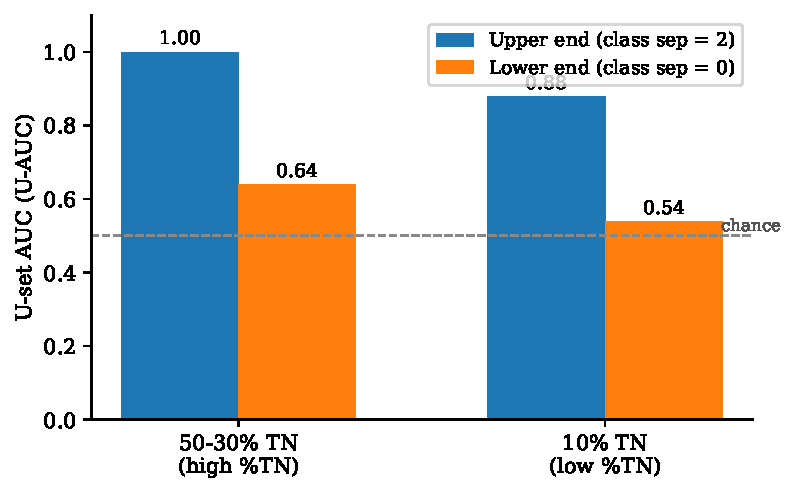
\includegraphics[width=0.70\textwidth]{figures/fig2_uauc.pdf}
\caption{Extremes of U-set AUC across synthetic hypercube class separations and true-negative proportions. At the 50/30\% true-negative regime, U-AUC ranged from 1.00 (class separation = 2) to 0.64 (class separation = 0). When the true-negative proportion fell to 10\%, U-AUC ranged from 0.88 to 0.54, approaching the chance level (dashed line).}
\label{fig:uauc}
\end{figure}

% ----------------------------------------------------------------------
% Figure 3: Permutation-count ablation dataset -- U-AUC vs KP
% ----------------------------------------------------------------------
\begin{figure}[htbp]
\centering
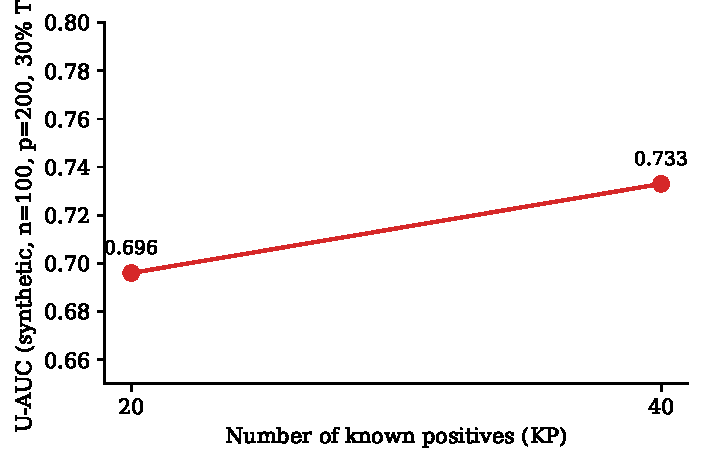
\includegraphics[width=0.60\textwidth]{figures/fig3_kp_uauc.pdf}
\caption{U-set AUC for the dimension-matched synthetic dataset (n=100, p=200, 30\% true negative, moderate hypercube separation) used in the permutation-count stability study. U-AUC = 0.696 at KP = 20 and 0.733 at KP = 40, spanning ``poor'' to ``acceptable'' discrimination.}
\label{fig:kp_uauc}
\end{figure}

% ----------------------------------------------------------------------
% Figure 4: Cliff's delta stability across permutation counts
% ----------------------------------------------------------------------
\begin{figure}[htbp]
\centering
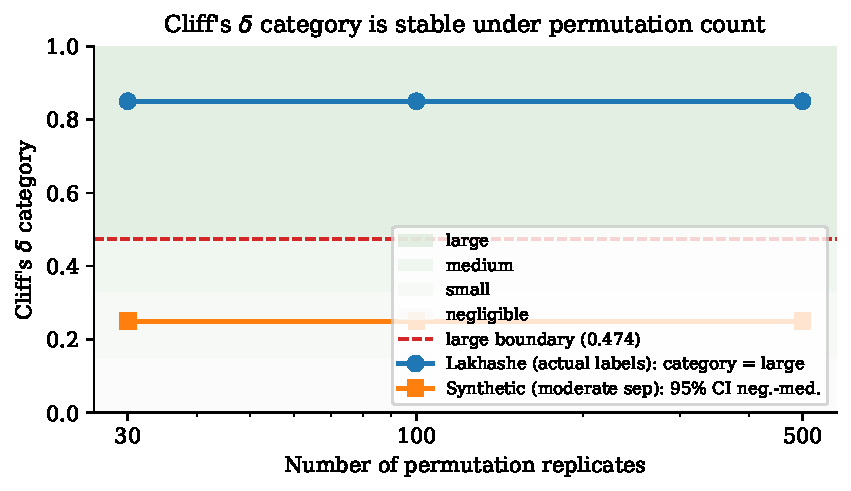
\includegraphics[width=0.78\textwidth]{figures/fig4_cliffs_stability.pdf}
\caption{Effect-size category of Cliff's $\delta$ is stable across permutation replicate counts. For the Lakhashe et al.\ dataset under actual P/U labels, the category remained ``large'' (Cliff's $\delta$ estimate $> 0.474$, dashed line) across 30, 100, and 500 permutation replicates. For the dimension-matched synthetic dataset with moderate separation, the 95\% CI spanned the negligible-to-medium range and was likewise unaffected by permutation count. The graded backgrounds indicate the standard Cliff's-$\delta$ effect-size bands (negligible, small, medium, large).}
\label{fig:cliffs}
\end{figure}

% ----------------------------------------------------------------------
% Figure 5: Dataset summary
% ----------------------------------------------------------------------
\begin{figure}[htbp]
\centering
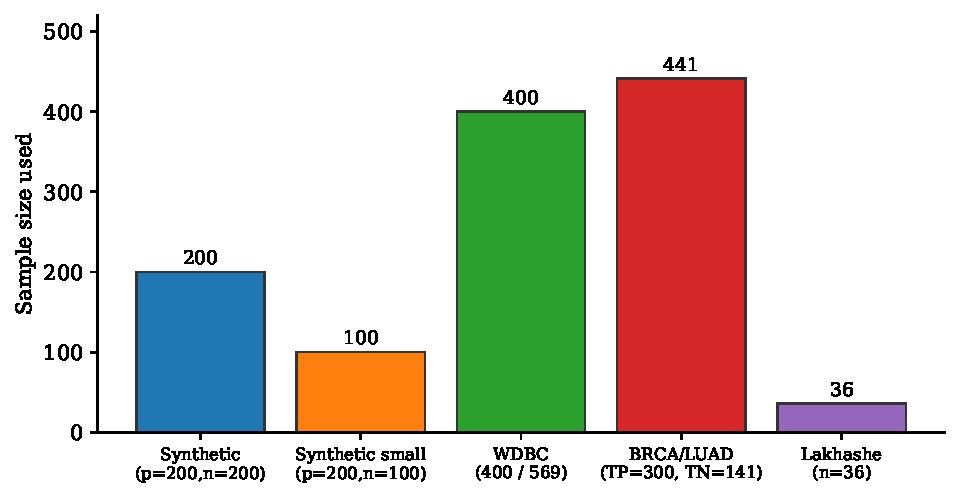
\includegraphics[width=0.82\textwidth]{figures/fig5_datasets.pdf}
\caption{Sample sizes of the benchmark datasets used. The synthetic datasets (200 features, 200 subjects or the 100-subject small variant) were generated with 30\% informative and 70\% redundant features. WDBC sub-samples drew 400 of 569 available instances. The BRCA/LUAD PANCAN subset provided 300 BRCA and 141 LUAD samples; 325 principal components retained 95\% of the variance. The Lakhashe et al.\ dataset comprised 36 Rhesus Macaques.}
\label{fig:datasets}
\end{figure}
